\subsection{Inertial Measurement Unit (IMU) Operation}
With the rangefinder's data processing implementation completed, the data is ready to be offset based on the device's relative location and direction in space. This was done with the use of an Inertial Measurement Unit (IMU). An IMU is a device that measures linear and angular momentum, as well as the direction of the magnetic field at a point in space. It accomplishes this by reading data from an accelerometer, gyroscope, and magnetometer respectively. 

\subsubsection{Selection}
This project required a sensitive IMU that is able to provide data to tell compass direction and change of position. Due to the time limitations and budgetary restrictions of this project, we chose the PmodNAV IMU that provides 10-degree of freedom functionality through the LSM9DS1 3-axis accelerometer, 3-axis gyroscope, and 3-axis magnetometer, and the LPS25HB barometer \cite{lsm9ds1, lps25hd}. The PmodNAV is shown in Figure \ref{pmodnav}.

\begin{figure}[H]
	\centerline{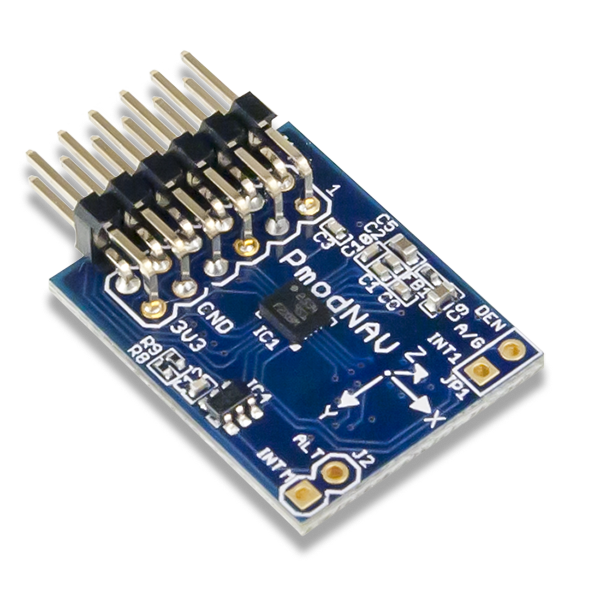
\includegraphics[width=0.5\textwidth]{pmodnav.png}}
	\caption{The PmodNAV 10-Axis IMU \cite{pmodnav_ref}}
	\label{pmodnav}
\end{figure}

The PmodNAV's simple Pmod connector made the IMU easy to integrate into this design, as it was fixed in position connected to the ZedBoard. Also, its communication was directly compatible with the ZedBoard, requiring no intermediate hardware.

\subsubsection{Communication}
The IMU supports two means of communication: Serial Peripheral Interface (SPI) and Inter-Integrated Circuit (I\textsuperscript{2}C) Communication \cite{lsm9ds1}. However the magnetometer on the LSM9DS1 is not addressable by the I\textsuperscript{2}C bus. Since the magnetometer was needed for its ability to tell compass direction, SPI communication was implemented. The magnetometer sensor SPI protocol is shown in Figure \ref{magnetometer_spi}.

\begin{figure}[H]
	\centerline{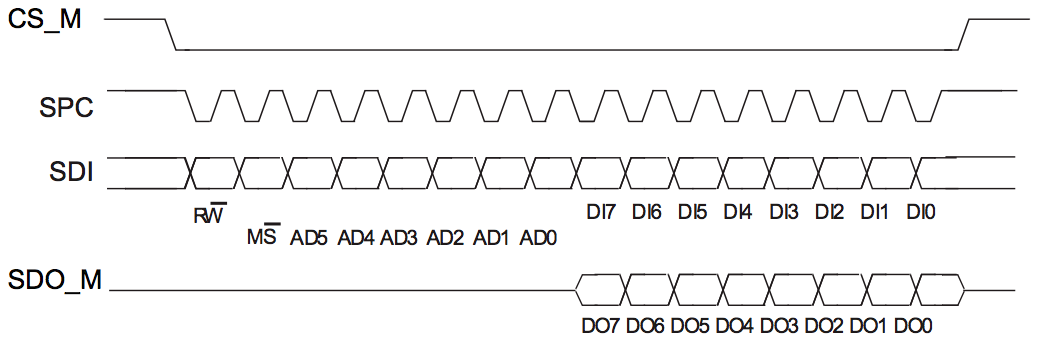
\includegraphics[width=1\textwidth]{magnetometer_spi.png}}
	\caption{Magnetometer SPI Read and Write Protocol \cite{lsm9ds1}}
	\label{magnetometer_spi}
\end{figure}

The CS\textunderscore{}M line is the magnetometer chip select and is an active low. It goes low at the beginning of the transaction and high at the end. The SPC is the clock controlled by the master. SDI and SDO\textunderscore{}M are the data input and data output lines, respectively. They are driven at the falling edge of SPC and should be captured at the rising edge \cite{lsm9ds1}.
\par
The register read and write commands are completed in 16 clock pulses. The first bit sent from the master, bit 0 or $R\overline{W}$, is the read/write bit. When data is read from the IMU this bit is set to 1, otherwise it is set to 0. When bit 1, the $M\overline{S}$ bit, is set to 1 the address is auto-incremented, allowing for multiple reads or writes to be completed in the same SPI transaction. Figure \ref{multiple_reads} shows a multiple-byte SPI read protocol. Bits 2-7, the $AD$ bits, are the address bits transmitted MSB first. When in write mode bits 8-15, the $DI$ bits, are the data that is written to the device MSB first. When in read mode bits 8-15, the $DO$ bits, are the data that is read from the device MSB first \cite{lsm9ds1}.

\begin{figure}[H]
	\centerline{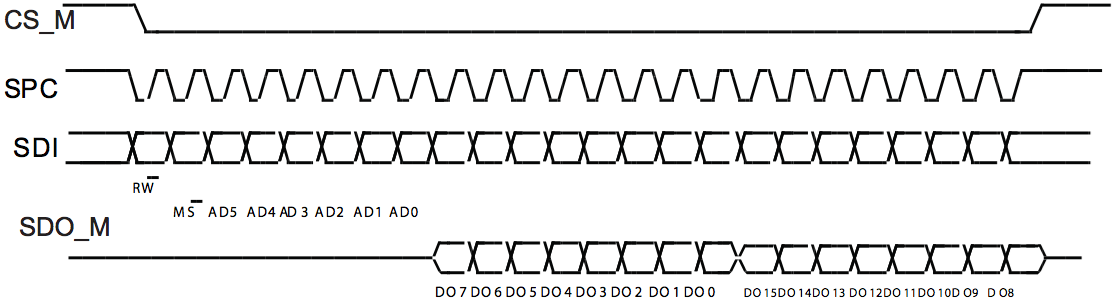
\includegraphics[width=1\textwidth]{multiple_reads.png}}
	\caption{Magnetometer Multiple-Byte SPI Read Protocol \cite{lsm9ds1}}
	\label{multiple_reads}
\end{figure}

\subsubsection{Register Settings} \label{imu_settings}
The LSM9DS1 IMU required memory register setting in order to turn on the magnetometer and function properly. The memory register settings were set by writing to the IMU in the SPI communication format shown in Figure \ref{magnetometer_spi}. For all of the settings adjustments the $R\overline{W}$ bit is set to 0, signifying a write command.
\par
One register that was written to was the magnetometer's control register 1, CTRL\textunderscore{}REG\textunderscore{}1\textunderscore{}M, which is at address 20\textsubscript{16}. 7C\textsubscript{16} was written to CTRL\textunderscore{}REG\textunderscore{}1\textunderscore{}M to signify ultra high performance mode for the magnetometer's x- and y-axis \cite{lsm9ds1}.
\par
The other register that was written to was the magnetometer's control register 3, CTRL\textunderscore{}REG\textunderscore{}3\textunderscore{}M, at address 22\textsubscript{16}. 80\textsubscript{16} was written to CTRL\textunderscore{}REG\textunderscore{}3\textunderscore{}M to turn off I\textsuperscript{2}C and turn on the magnetometer in the continuous-conversion mode \cite{lsm9ds1}.
\par
Due to time constraints, the magnetometer on the PmodNAV was the only slave that needed to be interfaced to. The accelerometer, gyroscope, and barometer were not used so the above registers only needed to set once.

\subsubsection{Read Registers}
With the magnetometer turned on and its registers set, its data was ready to be read. As such, the $R\overline{W}$ bit was set to 1. There are two registers that were read from in order to ensure data accuracy. 
\par
One register that was read from was the status register, STATUS\textunderscore{}REG\textunderscore{}M, which is at address 27\textsubscript{16}. This address was read from until the two least significant data bits read 11\textsubscript{2}, which signified that new x- and y-axis magnetometer data was ready. Once new x- and y-axis data was ready, the corresponding data registers were read from \cite{lsm9ds1}.
\par
The x- and y-axis data came in 16-bit resolution. Due to the SPI transfer protocol shown in Figure \ref{magnetometer_spi}, data was read 8 bits at a time MSB first. Since each axis had 16-bit resolution, each axis had two addresses containing 8-bit data words. The x- and y-data addresses are consecutive, so the 32 bits of data was obtained in one cascading read in the format shown in Figure \ref{multiple_reads}. Because of this, we performed a cascading read from address 28\textsubscript{16}, OUT\textunderscore{}X\textunderscore{}L\textunderscore{}M, to obtain the x-axis lower word, the x-axis upper word, the y-axis lower word, and then the y-axis upper word \cite{lsm9ds1}.







